\chapter{Teoretická část}

%%%%%%%%%%%%%%%%%%%%%%%%%%%%%%%%%%%%%%%%%%%%%%%%%
\section{Grafové databáze}

Grafy jsou velice přirozeným způsobem reprezentaci dat, zvláště v době, kdy většina dat je vytvářena uživateli a není strukturovaná. Grafy pomocí uzlů a hran přirozeně popisují objekty a vztahy mezi nimi, nevynucují náročné datové modelování skutečnosti do složitých datových struktur a usnadňují tak proces objevování informací v datech. Díky tomu, že grafy umožňují jednoduché prohladávání objektů, které mezi sebou mají vztahy (uzlů propojených hranami), jsou operace tohoto typu nad grafy relativně (například vůči relačním databázím) rychlé. 

Grafové databáze umožňují data reprezentovaná grafem ukládat a procházet tak, aby byly tyto přirozené výhody grafů zachovány a v některých případech byly také zajištěny některé vlastnosti relačních databázových systémů (jako například atomicitu transakcí). Problémů, pro které je vhodné využití grafových databází je mnoho, příkladem může být ochrana proti podvodům v bankovním sektoru. Některé vzorce v datech je složité odhalit pomocí modelů relačních databází. Grafové databáze naopak přináší nový pohled na data a implicitně ukazují vztahy mezi nimi. Umožňují tak odhalit v datech více podezřelých vzorců, které často mohou znamen právě bankovní podvody.\cite{Webber17} Dalším z mnoha příkladů jsou také řešení v oblasti \textit{data lineage}, která si kladou za cíl sledovat vztahy mezi daty společností a mapovat proces jejich zpracování. 

Tato kapitola má za cíl představit základní principy grafových databází. Popisuje reprezentaci grafů v databázi, možnosti analýzy dat a rozhraní, kterých je k tomu možné použít.

\subsection{NoSQL}
\label{sec:gdb-nosql}
NoSQL databázové sice nejsou předmětem této práce, grafové databáze nicméně bývají zařazovány jako podkategorie NoSQL a proto zde základní principy této skupiny technologií popíšeme. Samotná zkratka NoSQL je vykládaná různě, většinou jako \textit{"Not only SQL"} \cite{Evans09} a vykládá se jako označení pro databáze nerelačního typu určené pro zpracování \textit{Big Data}\footnote{Big Data jsou soubory dat velkého objemu, velké rychlosti a/nebo velké různorodosti, která vyžadují nové formy zpracování pro umožnění lepšího rozhodování, většího porozumění domény a optimalizace procesů.\cite{Laney01}}. Mezi hlavní uváděné výhody NoSQL databází patří: 

\begin{itemize}
  \item{\textit{Škálovatelnost:}} Zatímco klasické databázové systémy využívají \textit{vertikální škálovatelnost}\footnote{Vertikální škálování je prováděno pomocí navýšení zdrojů (ať už výpočetní kapacity, nebo paměti) jednoho zařízení.}, NoSQL databáze umožňují efektivní \textit{horizntální škálování}\footnote{Systém je horizontálně škálovatelný, jestliže lze navýšit jeho výkon a/nebo kapacitu přidáním dalšího zařízení. Jedná se tedy o síť spolupracujících zařízení.}. Data v NoSQL databázích bývají tedy typicky distribuovaná na několik uzlů\footnote{Pojem sluster může mít několik významů, zde je požíván jako množina síťově propojených počítačů.} a jejich zpracování tak může probíhat paralelně. 
  \item{\textit{Efektivní čtení:}} NoSQL datatabáze jsou silně orientovány na rychlé čtení (koncept \textit{write once, read many times}). Ve většině již nejsou data po zapsání do databáze nikdy modifikována, pouze nad nimi jsou vykonávány analýzy (dotazy). Za cenu potenciálně pomalejšího zápisu dat do databáze (který nám nevadí) získáme tedy výrazně vyšší rychlost čtení dat.  
  \item{\textit{Flexibilní datový model:}} NoSQL databáze buď nevyžadují žádné datové schéma, nebo je schéma volné (a lze ho tedy upravovat bez nutnosti úpravy stávajících dat). Dodržování schématu dat je tedy na aplikaci, která NoSQL databázi používá.  
  \item{\textit{Ekonomická stránka:}} jak již bylo uvedeno, relační databáze je nutné typicky škálovat vertikálně a to je nákladné\footnote{Jsou navyšovány prostředky jednoho stroje, což má technická omezení a čím více se těmto omezením blížíme, tím je škálování dražší. Vedlejším efektem této skutečnosti je často takzvaný \textit{vendor-locking}, tedy situace, kdy jsme nuceni používat specifický hardware (často od jedné konkrétní společnosti), který je velmi nákladný.}. Na druhé horizontální škálování je relativně levné - škáluje se přidáním nového uzlu. Vzhledem k tomu, že NoSQL databáze nevyžadují žádný konkrétní hardware, je možné používat takzvaný \textit{komoditní hardware} (uzly nemusí být hardwarově homogenní), který je levný.  
\end{itemize}

Aby těchto výhod NoSQL databáze dosáhly, využívají různé přístupy k reprezentaci dat a manipulaci s daty. Jejich hlavní rozdělení je následující: 

% Typy NoSQL databází
\begin{itemize}
  \item{\textit{Databáze typu klíč-hodnota:}} Tyto databáze mají zcela volné datové schéma, jsou realizovány jako mapa klíčů a hodnot. Hodnota přitom typicků může nabývat několika datových typů (například číslo, text, binární řetězec, kolekce některého z předchozích). Operace nad tímto uložištěm jsou poměrně jednoduché a zpravidla neposkytují pokročilé nástroje pro analýzu dat na základě obsahu - pouze na základě klíče. Příklady tohoto typu databází jsou Redis\footnote{https://redis.io/}, Riak\footnote{http://basho.com/products/}, nebo Voldemort\footnote{http://www.project-voldemort.com/voldemort/}.
  \item{\textit{Dokumentová databáze:}} Dokumentové databáze ukládají a spravují zpravidla strukturované dokumenty. Nejčastější formáty dokumentů jsou \textit{\nomExpl{JSON}{JavaScript Simple Object Notation}} a \textit{\nomExpl{XML}{Extensible Markup Language}}. Narozdíl od databází typu klíč-hodnota umožňují dokumentové databáze přistupovat k dokumentům a analyzovat je dle jejich obsahu. Příkladem mohou být MongoDB\footnote{https://www.mongodb.com/} a CouchDB\footnote{http://couchdb.apache.org/}.  
  \item{\textit{Sloupcové databáze:}} Sloupcové databáze se skládají z tabulek, ve kterých může mít každý řádek libovolný počet sloupců (nezávislý na ostatních řádcích). Volné vkládání sloupců sloupců nijak nesnižuje výkon sloupcových databází, které bývají masivně distribuované. Příklady sloupcových databází jsou HBase\footnote{https://hbase.apache.org/}, BigTable\footnote{https://cloud.google.com/bigtable/} a Cassandra\footnote{http://cassandra.apache.org/}.
  \item{\textit{Grafové databáze:}} Konečně posledním a pro nás nejzajímavějším typem NoSQL databází jsou grafové databáze. Tyto databáze jsou určené pro data, která je vhodné modelovat a dotazovat jako grafy (viz. kapitola \ref{sec:gdb-grafy}). Vnitřní reprezentace grafů může být různá podle toho, pro jaký typ grafových úlovh je daná databáze primárně určena. Konkrétní databáze budou popsány v kapitole \ref{sec:gdb-databaze}.
\end{itemize}


\subsection{Grafy}
\label{sec:gdb-grafy}
% Matematická definice
Ještě před popisem vlastních grafových databází blíže popíšeme grafy jako takové a jejich typy. Nejdříve uvedeme základní matematický rámec teorie grafů, se kterým budeme dále pracovat. 

Graf \textit{G} je trojice \textit{G = (V, E, $\epsilon$)}, kde \textit{V} je množina vrcholů\footnote{nebo také uzlů} a \textit{E} množina hran. \textit{$\epsilon$} je přiřazení, které každé hraně přiřazuje: 
\begin{itemize} 
	\item{} množinu dvou vrcholů (koncové vrcholy) pro \textit{neorientovaný graf}.
	\item{} uspořádanou dvojici vrzcholů (počáteční a koncový vrchol) pro \textit{orientovaný graf}.
\end{itemize}

% Multigrafy / prosté grafy
Pokud graf neobsahuje paralelní hrany\footnote{nebo také multihrany}, tedy hrany, které mají stejné počáteční a koncové vrcholy (orientovaný graf), respektive stejné koncové vrcholy (neorientovaný graf), je označován jako \textit{prostý graf}. Naopak pokud graf paralelní hrany obsahuje, je označován jako \textit{multigraf}.\cite{Demlova17}

% Labeled grafy
Grafy z pohledu informačních technologií matematickou definici grafu dále rozšiřují. Umožňují definovat typy hran a uzlů, čímž vzniká \textit{ohodnocený graf}\footnote{Opakem ohodnoceného grafu je jednovztahový nebo také homogenní graf.} Například ohodnocený graf na obrázku \ref{fig:labeled_graf} obsahuje dva typy uzlů (:OSOBA a :ČLÁNEK) a dva typy hran (:ZNÁ a :ČETL).

\begin{figure}
\begin{center}
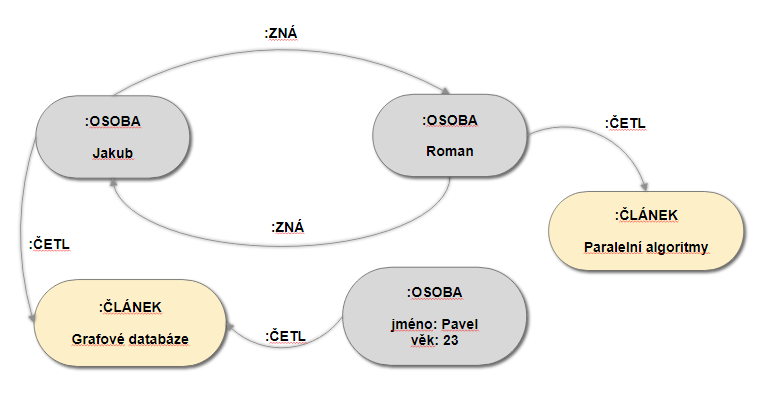
\includegraphics[width=14cm]{figures/labeled_graph}
\caption{Ohodnocený graf}
\label{fig:labeled_graf}
\end{center}
\end{figure}

% Property grafy
Ohodnocené grafy sice poskytují možnost rozlišit typy hran a uzlů, v mnoha situacích je ale žádoucí zachytit do grafu více informací. \textit{Atributové grafy} umožňují přiřadit hranám a uzlům libovolný počet atributů (dvojic klíč-hodnota), které obsahují informace o daném uzlu, respektive hraně. Příkladem může být věk osob, či datum vydání článku (viz obrázek \ref{fig:property_graf}). Většina grafových databází pracuje právě s atributovými grafy.\cite{Lal15}

\begin{figure}
\begin{center}
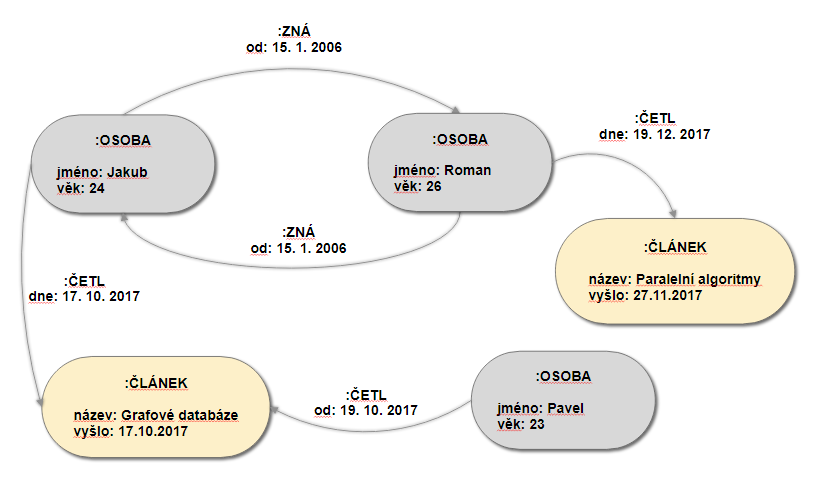
\includegraphics[width=14cm]{figures/property_graph}
\caption{Atributový graf}
\label{fig:property_graf}
\end{center}
\end{figure}

% Hypergrafy
Generalizací grafu je tzv. \textit{hypergraf}. Ten se proti grafu liší tím, že zatímco hrana grafu vede mezi právě dvěma vrcholy, hyperhrana (tedy hrana v hypergrafu) je mnoužinou jednoho a více vrcholů.\cite{Diestel00} Hypergrafy jsou používány k reprezentaci dat v mnoha oborech a některé GDB je přímo podporují (například HypergraphDB\footnote{http://hypergraphdb.org/}).


\subsection{Perzistence}
Aby bylo možné v dalších kapitolách popsat pokročilé aspekty \nom{GDB}{grafových databází} (jako například indexování, či transakce), je nejdříve nutné popsat jejich základní principy. Nutnost ukládat data ve formě grafů je starší než grafové databáze samotné, existuje tak mnoho způsobů uložení grafů z nichž ty nejběžnější zde popíšeme. Ještě předtím je nutno poznamenat, k jakým typům úloh jsou grafové databáze zejména využívány. Základními grafovými úlohami jsou \nomExpl{BSF\footnote{Breadth-first search}}{průchod do hloubky} a \nomExpl{DFS\footnote{Depth-first search}}{průchod do šířky}. Oba tyto algoritmy musí projít v nejhorším případě\footnote{Pro konkrétní problémy jsou často \nom{BFS} a \nom{DFS} algoritmy upravovány tak, aby bylo možné některé větve průchodu tzv. ořezávat - tedy procházet pouze jejich část, nebo je neprocházet vůbec.} všechny hrany a uzly grafu, je tedy vidět, že pro efektivitu grafových databází je klíčová rychlost přechodu z jednodoho uzlu do (všech) jeho sousedních uzlů pomocí existujících hran.

% RDBMS reprezentace
Než se pustíme do popisu nativních grafových uložišť, krátce popíšeme možnost ukládání grafů pomocí relačních databází. Jedním z možných řešení může být dvojice tabulek \textit{UZLY} a \textit{HRANY}. Tabulka uzlů by obsahovala identifikátor uzlu a případné další parametry uzlu, tabulka hrany by obsahovala referenci na počáteční a koncový uzel hrany a případné další parametry hrany\footnote{V tomto případě předpokládáme orientovaný prostý atributový graf, pro jiné grafy by bylo nutné tuto strukturu upravit (což ale není těžké). Například v případě ohodnoceného grafu je možné uvažovat separátní tabulku pro každý typ uzlů.}. Všechny hrany daného uzlu je tedy možné získat pomocí spojení těchto tabulek pomocí cízího klíče, složitější průchody potom mohou být docíleny pomocí relace tabulky hran na sebe sama. Problém tohoto přístupu je nutnost rekurzivních operací \textit{join} a jejich vysokých nákladů\footnote{Spojování tabulek pomocí cizích klíčů je jedna z nejdražších operací ve světě relačních databází.}. Tyto problémy mohou být částečně eliminovány použitím sloupcových či dokumentových NoSQL databází. Přestože v takovém případě nejsou používány rekurzivní operace spojování tabulek (ve světě NoSQL tato operace neexistuje), je k datům přistupováno pomocí prohledávání indexů a operace je tak stále výrazěn dražší, než při použití nativního grafového uložiště.\cite{Lal15} 

% Matice sousednosti
Nejzákladnější nativní reprezentací grafu je tzv. \textbf{matice sousednosti}. Ta využívá možnosti reprezentování hran grafu jako dvojice uzlů a reprezentuje graf jako matici \textit{M} o rozměrech \textit{|V|x|V|}, kde \textit{|V|} je počet uzlů grafu. Pokud existuje mezi uzly \textit{i} a \textit{j} hrana, pak bude \textit{M\textsubscript{i,j} != 0}. 
Pokud nás zajímá pouze existence hrany, nabývá matice pouze hodnot \textit{\{0, 1\}}. Pokud jsou hrany ohodnocené, pak nenulová hodnota buňky na dané pozici ukazuje nejen existenci hrany mezi danými uzly, ale také její ohodnocení. Pro neorientovaný graf je matice symetrická. Pokud je graf orientovaný, potom \textit{M\textsubscript{i,j}} určuje existenci hrany z uzlu \textit{i} do uzlu \textit{j} a \textit{M\textsubscript{j,i}} naopak existenci hrany z uzlu \textit{j} do uzlu \textit{i}. 
Tato reprezentace grafu zajišťuje vysokou efektivitu přidávání, odstraňování a kontroly existence hran - tyto operace jsou okamžité.  Na druhou stranu přidání nového uzlu do grafu je nákladná operace, matice musí být přealokována a překopírována. Vzhledem k tomu, že paměťová náročnost matice sousednosti je kvadratická vzhledem k počtu uzlů a nezávisle na počtu hran (není tedy vhodná pro řídké matice\footnote{TODO poznámka o tom, že řídké matice jsou what u need}), je drahé i její překopírování. 
Pro nalezení všech sousedních uzlů je nutné všechny uzly projít a zkontrolovat, zda hrana existuje, či nikoliv. Hledání sousedních uzlů je nejčastější operací při průchodu grafu, tato reprezentace tedy není vhodná ani na složitější průchody.

% Laplaceovská matice
Speciální variantou matice sousednosti je \textbf{Laplaceovská matice}. Ta má stejně jako matice sousednosti rozměry \textit{|V|x|V|}. Diagonála Laplaceovské matice ukazuje stupeň vrcholu a pokud existuje mezi dvěmi vrcholy hrana, je hodnota matice na dané pozici \textit{-1}. Pokud mezi vrcholy hrana naní, hodnota je \textit{0}. Hlavní výhodnou reprezentace grafu Laplaceovskou maticí je umožňění spektrální analýzy grafu\cite{Barnard93}, kdy jsou pomocí vlastních čísel matice analyzovány vlastnosti grafu.

% Matice incidence
Další možnou maticovou reprezentací grafu je \textbf{matice incidence}. Jedná se o dvoudimenzionální matici o rozměrech \textit{|V|x|E|}, kde každý sloupec matice odpovídá jedné hraně a řádek jednomu uzlu. Pokud je uzel \textit{v} účastníkem hrany \textit{e}, potom \textit{M\textsubscript{v,e} != 0}. Pokud se jedná o neorientované grafy, nabývá matice pouze hodnot \textit{\{0, 1\}}. Pokud je graf orientovaný, potom je odchozí hrana kódována jako \textit{-1} a příchozí jako \textit{1}. V případě ohodnoceného grafu mohou být hodnoty obecně všechna celá čísla (podobně jako u matice sousednosti), přičemž opět platí, že záporné číslo značí odchozí hranu a kládné číslo příchozí. Vzhledem k tomu, že pro většinu grafů platí, že počet hran \textit{|E|} je vyšší než počet uzlů \textit{|V|} (často, například u sociálních sítí, je výrazně vyšší), je tato reprezentace pro svou vysokou paměťovou náročnost ve většině případů nevhodná. Narozdíl od ostatních reprezentací ale umožňuje ukládání hypergrafů (hrany hypergrafu mohou zahrnovat libovolný počet vrcholů). Zatímco u běžného grafu by každý sloupec matice incidence obsahoval právě dva nenulové prvky, u hypergrafu jich může být libovolný počet.

% List sousednosti 
Některé problémy matice sousednosti řeší \textbf{list sousednosti}. Ten je implementován jako množina listů, kde každému uzlu připadá jeden list sousedních uzlů. Paměťová náročnost této reprezentace je tedy \textit{|V|+|E|}, kde \textit{|V|} je počet uzlů a tedy počet listů sousednosti a \textit{|E|} je počet hran a tedy celkový počet prvků obsažených v listech sousednosti. List sousednosti je výrazně úspornější reprezentací grafu z paměťového hlediska než je matice sousednosti a je tedy vhodný i pro řídké grafy. Zároveň umožňuje rychlé nalezení všech sousedních uzlů pro daný uzel, v listu jsou vypsány pouze ty uzly, se kterými je uzel propojen a procházení grafu je tak rychlé. Přidání hrany do grafu je přidáním jednoho prvku do listu (respektive dvou listů v případě neorientovaného grafu) a přidání uzlu je také relativně efektivní - znamená vytvoření nového listu a přidání ho do množiny ostatních listů. Drahé jsou naopak operace odebrání hrany (je nutné projít všechny sousedy obou koncových uzlů hrany) a odebrání uzlu (je nutné projít všechny hrany). Také ověření existence konkrétní hrany je relativně drahé (je potřeba opět projít všechny sousedy daného uzlu). Toto může být řešeno alternativní implementací, napříkald mohou být listy sousedů řazeny. Tím se sice sníží složitost ověření existence hrany, ale zvýší se složitost přidání nové hrany.
Při reprezentaci velkých grafů pomocí listů sousednosti se používají kompresní techniky, díky kterým je možné dále snižovat paměťovou náročnost.\cite{Boldi04} 

% TODO reprezentace grafu jako RDF (haxtree, bitmap). 

% TODO obrázky k reprezentaci grafů

Důležitým kritériem pro výběr reprezentace grafu je \textit{lokalita dat}. Cílem je uložit graf tak, aby jejich fyzické umístění odpovídalo jejich logické vzdálenosti a při průchodu grafem tak byla data pro další krok načtena co nejrychleji. K dosažení optimality lokality dat reprezentovaných grafem existuje mnoho technik, vzhledem k tomu, že se ale jedná o \textit{NP-těžkou} úlohu, jedná se často o heuristiky a aproximační algoritmy. Některé z používaných metod jsou například metoda minimalizace šířky matice autorů \textit{Cuthill a McKee} \cite{Cuthill69}, \textit{rekurzivní spektrální bisekce} \cite{Barnard93}, nebo metoda založená na průchodedech grafu do šířky (BFSL\footnote{Breadth First Search Layout}) \cite{Furaih98}.


\subsection{Typy dotazů}
\label{sec:gdb-dotazy}

% Traversal pattern
Na rozdíl od indexově náročných množinových operací relačních databází využívají grafové databáze bezindexové místní prohledávání (traverzování).\cite{Anglels08} Relační databáze obsahují data typicky v normalizované formě v několika separátních tabulkách tak, aby bylo zamezeno duplikaci dat. Řádky těchto tabulek mohou být chápány jako objekty popsané svými vlastnostmi. Vztahy mezi objekty jsou definovány primárními a cizími klíči a musí být při dotazování explicitně vytvořeny spojením tabulek pomocí \textit{join} operace. Jak vyhledávání záznamů v tabulkách, tak spojování tabulek je (v ideálním případě) realizováno pomocí vyhledávacích indexů, které časovou složitost těchto operací značně snižují, obecně ale ne dostatečně. Databázové vyhledávací indexy jsou typicky realizovány pomocí vyhledávacích stromů (konkrétně B-stromů \cite{Leach05}), vyhledání zánamu má tedy logaritmickou časovou složitost vzhledem k počtu uzlů\footnote{Konkrétně operaci vyhledání uzlu má složitost \textit{$\Theta$(b log$_b$(n))} a operace vyhledání rozsahu uzlů \textit{$\Theta$(b log$_b$(n) + k/b)}, kde \textit{n} je počet uzlů, \textit{b} je úroveň stromu a \textit{k} je velikost rozsahu.\cite{Cormen09}}. 
Grafové databáze na druhé straně obsahují typicky pouze jednu strukturu - graf\footnote{Grafové databáže mohou obsahovat jeden velký graf, nesouvislý graf, nebo množinu grafů. Z hlediska této práce je toto ale technický detail a pokud nebude explicitně řečeno jinak, budeme předpokládat, že grafová databáze obsahuje jeden velký graf.}. Ten ve své fyzické reprezentaci obsahuje všechny své hrany, vztahy mezi objekty (vrcholy) v grafu jsou tedy implicitní, není potřeba je při každém dotazu vytvářet. Tato skutečnost s sebou nese výhody i nevýhody. Jednou z podstatných nevýhod je složitost rozdělení grafu na podgrafy a tedy obtížná distribuce grafu (popsáno v kapitole \ref{sec:gdb-distribution}). Naopak výhodou je instantní čas, ve kterém je možné se v grafu posouvat mezi sousedními uzly. To je natolik výraznou vlastnostní grafových databází, že výrazně ovlivňuje způsob, jakým je přistupováno k datům v grafových databázích. Tím nejčastějším je právě průchod grafem (traverzování, nebo také \textit{Traversal pattern}). 

Na začátku průchodu grafu jsou pomocí indexu vyhledány výchozí uzly, ze kterých bude graf procházen. Z nich se dotaz pohybuje po grafu pomocí sousedních hran a uzlů dle zadaných kritérií. Těmi jsou typicky typy hran a uzlů, podmínky na jejich vlastnosti (uvažujeme atributový graf, viz kapitola \ref{sec:gdb-grafy}) a hloubka prohledávání. Součástí definice dotazu je také zvolení typu průchodu - průchod do hloubky (\textit{\nom{DFS}{Depth-first search}}, nebo průchod do šířky (\textit{\nom{BFS}{Breadth-first search}}. Když jsou projity všechny cesty odpovídající zadaným kritériím, jsou vráceny uzly, ve kterých průchod skončil. Typickými úlohami řešenými pomocí průchodů grafem je například zjištění existence cesty mezi dvěma uzly, nalezení nejktraší cesty, nalezení všech cest a uzlů odpovídajícíh zadaným kritériím apod.  

% TODO příklad traversalu

% Dotazy na podgraf, nadgraf, podobný graf
Dalšími typy dotazou kromě obecného průchodu gravu jsou \textit{dotazy na podgrafy}, \textit{dotazy na nadgrafy} a \textit{dotazy na podobné grafy}. Zadáním těchto dotazů je také graf, označme \textit{$G_dotaz$}. Tento dotazový graf může obsahovat uzly a hrany, u kterých nejsou specifikovány bližší vlastnosti, v grafu může být určena množina přípustných typů uzlů a hran, nebo například maska jejich typů. Dotazy na podgrafy hledají specifický vzor grafů v grafové databázi - v databázi jsou vyhledávány všechny grafy, který \textit{$G_dotaz$} obsahují. V případě dotazu na nadgraf naopak hledáme v databázi všechny datové grafy, které jsou v \textit{$G_dotaz$} obsaženy. U dotazů na podobné grafy je výsledek dotazu vyhodnocován pomocí metriky podobnosti.\cite{Koutra11} Tyto typy dotazů jsou vyhodnocovány ve třech krocích: 

\begin{enumerate}
	\item{Extrakce:} Z grafu \textit{$G_dotaz$} jsou vyextrahovány indexované charekteristiky (stejným způsobem jako z datových grafů).
	\item{Filtrace:} Porovnáním vyextrahovaných charakteristik jsou z datových grafů vybrány ty, které odpovídají charakteristikám \textit{$G_dotaz$}. Tím vznikne množina kandidátů na výsledek, přičemž cílem indexační techniky je, aby tato množina obsahovala co nejmenší počet falešně pozitivních kandidátů. Pokud by množina neobsahovala žádné falešně pozitivní kandidáty (indexační technika by měla dostatečnou filtrační schopnost), byla by tato množina rovna množině výsledných grafů (a nebylo by nutno provádět třetí fázi). 
	\item{Verifikace:} Grafy z množiny kandidátních řešení jsou podrobně porovnány s \textit{$G_dotaz$}, čímž jsou vyloučeni případní zbylí falšeně pozivní kandidáti a dostáváme množinu skutečných výsledků. 
\end{enumerate}

Je zjevné, že tyto typy dotazů jsou velmi závislé na konkrétních indexačních technikách, ty jsou popsány v kapitole \ref{sec:gdb-indexy}.

% TODO příklad dotazu na podgraf, nadgraf

%TODO
\subsection{Indexy}
\label{sec:gdb-indexy}
% Indexování uzlů a hran
Stejně jako je tomu u relačních databází, i ve světě grafových databází se hojně používají indexy (a také už byly v předchozím textu několikrát zmíněny) a je jich hned několik typů. Průchody (\textit{traverzování}) grafem používají pouze základní indexy a to ve chvíly, kdy jsou hledány výchozí uzly. Konkrétní databáze můžou k indexům přistupovat specifickým způsobem, je tedy vhodné si u každé databáze ověřit, co je automaticky indexováno. Zpravidla je žádoucí indexovat typy (\textit{labely}) a vybrané atributy hran a uzlů. Například pokud by existoval index na typ uzlů a chtěli bychom v grafu o milionu uzlů vyhledat všechny uzly typu \textit{:OSOBA} (a z nich graf procházet), databáze by neprocházela všechny uzly, ale podle indexu by vyhledala přesně uzly tohoto typu. Tyto základní indexy si můžeme představit jako indexy které známe z relačních databází, tedy jako B-stromy a jim podobné struktury\footnote{Implementace indexu v Neo4J (\textit{GB+Tree}): \url{https://github.com/neo4j/neo4j/blob/3.4/community/index/src/main/java/org/neo4j/index/internal/gbptree/GBPTree.java}}.

% indexační metody pro dotazy na podgraf (mining a non-mining based)
U strukturálních dotazů je situace komplikovanější. V případě \textit{dotazů na podgrafy} se indexační metody dělí na tzv. \textit{mining based} (indexy založené na dolování dat (\textit{data mining})) a \textit{non-mining based}. \textit{Mining based} indexační metody jsou založené na pozorování, že pokud množina vlastností grafu \textit{$G_dotaz$} není obsažena v některém z datových grafů, nebude takový datový graf obsahovat ani celý dotazový graf. Stačí tedy vybrat vhodné podstruktury grafu \textit{$G_dotaz$} a vyhodnocovat dotazy pouze na nich (typicky se jedná o časté podstromy či podgrafy). Pro tyto podmnožiny vlastností je vytvořen \textit{invertovaný index}\footnote{TODO vysvětlit invertovaný index} a při vyhodnocování grafu \textit{$G_dotaz$} jsou nejdříve identifikovány a vyhodnoceny tyto struktury, čímž je získána množina kandidátů. Nevýhodou tohoto přístupu je závislost \textit{invertovaného indexu} na jak datových, tak dotazových datech. Pokud se výrazně změní typ dotazových grafů, nebo se změní datové grafy tak, že vybrané podstruktury již nemají potřebnou filtrační schopnost, je nutné přeindexovat. Mezi \textit{mining based} indexační metody patří například \textit{GIndex} \cite{Yan04} a \textit{TreePI} \cite{Zhang07}. \textit{Non-mining based} indexační metody naopak indexují grafy jako celek, neanalyzují jejich strukturu nabo časté vzory. Nejsou tak závislé na dotazových ani datových grafech, nedosahují ovšem takové filtrační schopnosti jako \textit{mining based} metody a tím pádem vyžadují delší fázi verifikace. Patří mezi ně \textit{GraphGrep} \cite{Giugno02}, \textit{GDIndex} \cite{Williams07}, \textit{GString} \cite{Jiang07} a \textit{GraphREL} \cite{Sakr09}.

% TODO indexační metody pro dotazy na nadgraf a podobný graf

% TODO fultextové indexy

%TODO doplnit
\subsection{Transakce}

%ACID
Pojďme nejprve připomenout standardní transakční model světa relačních databází - \textbf{ACID}. Tento model říká, že transakce v databázovém systému musí být atomické (\textit{\textbf{A}tomocity}, tedy nedělitelné. Pokud tedy selže některá z operací transakce, selže celá transakce a je proved její \textit{rollback}\footnote{Rollback transakce je událost, která nastává, pokud transakce selže, nebo pokud je uživatelem explicitně vyvolána. Všechny kroky, které byly v rámci transakce provedeny jsou vráceny, po rollbacku transakce je tedy databáze ve stejném stavu, jako před spuštěním transakce. Opakem rollbacku je operace \textit{commit}, která potvrzuje všechny změny provedené v transakci.}. Nemůže se tedy stát, že by byla provedena jen část operací transakce a databáze se ocitla v nekonzistentním stavu. Jinými slovy, po provedení jakékoliv transakce (úspěšném i neúspěšném) bude databáze vždy konzistentní (\textit{\textbf{C}onsistency}). Všechny transakce jsou také izolované (\textit{\textbf{I}solated}), tedy transakce jsou na sobě navzájem nezávislé a neovlivňují si navzájem data. V případě, že dojde ke konfliktu několika transakcí, databázový systém konflikt vyřeší tak, aby byla tato vlastnost zachována\footnote{Existuje několik stuňu izolace transakcí , výčtem \textit{read uncommitted}, \textit{read committed}, \textit{repeatable read} a \textit{serializable}. Právě na úrovni izolace konfliktujících transakcí záleží, jakým způsobem bude konflikt vyřešen. Toto téma je podrobně rozebráno napříkald v TODO}. A konečně poslední vlastností transakcí v transakčním modelu ACID je trvanlivost (\textit{\textbf{D}urability}). Tato vlastnost zajistí, že změny provedené transakcí jsou trvalé. 

%BASE
Vlastnosti ACID transakčního modelu jsou klíčové pro relační databázové systémy, které mají širokou škálu využití. Pro svět NoSQL databází (do kterého bývají grafové databáze často řazeny) tento model ale není vhodný, a to především kvůli silnému důrazu na konzistenci dat a tedy jejich obtížné distribuovatelnosti\footnote{Distribuovanost dat je klíčová pro NoSQL databáze obecně, pro grafové databáze to ale ne vždy platí. Toto bude více rozebráno v kapitole \ref{sec:gdb-distribution}.}. Zaven je tedy alternativní transakční model - \textbf{BASE}. Ten říká, že systém numusí být nutně dostaupný vždy, stačí základní dostupnost (\textit{\textbf{B}asic \textbf{A}vailability}) - tedy dostupnost po většinu času. Mohou nastastat částečné výpadky, ale nikdy nedojde k výpadku celého systému\footnote{Tato vlastnost opět míří především na ty NoSQL databáze, které předpokládají vysokou distribuovanost dat a skládají se tedy z více uzlů. Od grafových databází, které distribuované nejsou očekáváme tedy dostupnost úplnou.}. Systém je v takzvaném volném stavu (\textit{\textbf{S}oft-state}), je dynamický, neustále docházi ke změnám. V případě distribuování a replikaci dat je důsledkem této vlastnosti mimo jiné to, že ne všechny repliky musí být nutně vzájemně konzistentní. A konečně, máme jistotu, že systém bude vždy "nakonec" uveden do konzistentního stavu (\textit{\textbf{E}ventual consistency}), ale nemusí být konzistentní v každém okamžiku. Například k vynucení konzistence může dojít až při čtení daty, při jejich zápisu nutná není\footnote{Jedná se o takzvanou \textit{lazy} konzistenci.}. Tento model tedy také umožňuje zachování jistoty konzistence dat, není ale automatická, jako tomu je u předchozího modelu. \cite{Sadalage13}

Jak už bylo zmíněno, grafové databáze jsou typem NoSQL databází. Přesto většina grafových databází není NoSQL databází v pravém smyslu slova. Výsledkem tak je, že některé grafové databáze plně podporují ACID transakční model, jiné naopak BASE. Toto je blíže diskutováno v popisu konkrétních grafových databází (kapitola \ref{{sec:gdb-databaze}}).

% TODO
% https://link.springer.com/chapter/10.1007/978-3-319-29919-8_8

% TODO zámky

\subsection{Distribuovatelnost}
\label{sec:gdb-distribution}
V kapitole \ref{sec:gdb-nosql} jsme zmínili, že distribuovanost dat je klíčovou vlastností NoSQL databází\footnote{Pokud je to možné, je vždy efektivnější když data distribuovaná nejsou. K jejich distribuování přikračujeme až ve chvíli, kdy nás k tomu nutí okolnosti - například velikost dat.}. Pro distribuci dat se využívá kombinování dvou technik - \textit{rozdělení (sharding)} a \textit{replikace} dat. 

% Sharding
Rozdělení dat je základním předpokladem pro jejich distribuci - musí dojít k rozdělení dat na vhodné množiny a ty uložit na různé uzly v clusteru. Při manipulaci s daty je tak přistopováno na jeden nebo více uzlů podle toho, jaká data jsou zpracovávána. Při rozdělování dat je bráno v potaz jejich rovnoměrné rozdělení, minimalizace počtu uzlů využívaných k provádění operací nad daty a optimalizace jejich fyzického rozmístění. 

% Replikace
Aby byla při případném výpadku části uzlů stále přístapná všechna data (všechny \textit{shardy}) jsou po částech mezi uzly několikrát replikována. Tím je zajištěno, že při selhání (ať už dočasném, nebo trvalém) jednoho uzlu nedojde ke ztrátě dat samotných, ani ke ztrátě přístupu k nim (pokud neselžou všechny repliky obsahující danou část dat). Počet, kolikrát jsou data v databázi replikována (replikační faktor) určuje mimo jiné algoritmus, pomocí kterého jsou data na repliky ukládána a rychlost jejich čtení. 

% Kontext grafů TODO
U grafových databází je ale distribuce dat (a tedy horizontální škálování) výrazně komplikovanější, než u ostatních NoSQL databází. Data v nich jsou uložena do několika několika struktur (tabulek, dokumentů, dvojic klíč-hodnota), zatímco obsahem grafové databáze je typicky pouze jediná struktura - graf. Rozdělení grafu na podgrafy je obtížný problém (zvláště pokud se jedná například o úplný graf), proto obecně ne mnoho grafových databází tuto možnost vůbec umožňuje. Přesto existují metody, které se distribucí grafu zabývají. Výsledná distribuce je potom optimální pouze pro podmnožinu grafových úloh (například průchod do šířky, hledání nejmenší kostry atd.). Distribucí grafu na několik uzlů se mění čas, v jakém je možné získat seznam sousedních vrcholů grafu v případech, kdy hrana mezi vrcholem a jeho sousedem spojuje dva podgrafy na dvou různých uzlech, je tedy obtížné graf distribuovat při snaze zachovat co nejvyšší rychlost průchodu grafem. Příkladem algoritmů pro rozdělení grafu může být \textit{1D dělení} a \textit{2D dělení} matice sousednosti \cite{Yoo05}, nebo mnoho technik aproximujících \textit{optimální k-rozdělení grafu}\footnote{Optimální bisekce grafu je NP-obtížný problém \cite{Garey90}, tedy i optimální k-rozdělení grafu je nejméně NP-obtížný problém. Proto jsou používány aproximační algoritmy.}.\cite{George78} \cite{Fiduccia82} \cite{Battiti99}


%TODO 
\subsection{Databáze - příklady}
\label{sec:gdb-databaze}

% TODO Neo4J

% TODO Sparksee

% TODO InfiniteGraph

% OrientDB

% Titan

% JanusGraph

% HyperGraph DB

% Jena

%TODO 
\subsection{Dotazovací jazyky}

% API a REST API
Od roku 2004, kdy byla uvedena databáze Neo4J (TODO CITE) a tím začal boom grafových databází, nebyly zatím definovány standardy pro dotazování dat v grafových databázích. Existuje tak mnoho způsobů a nástrojů, které dotazování dat umožňují, v podstatě žádný ale zatím nelze nazývat standardem. Základním způsobem dotazování dat v kontextu grafových databází jsou programová rozhraní (API TODO odkaz na kapitolu), nebo případně REST API (todo odkaz) nezávislá na konkrétním programovacím jazyku. Dotazy jsou v tomto případě přímo součástí kódu aplikace a přímo z aplikace jsou volány, bez prostředníka. Jednoznačnou výhodou tohoto přístupu je, že tato API, která má každá grafová databáze své, podporují všechny funkce dané databáze. To je zároveň i hlávní nevýhodou - grafové databáze fungují na různých, často protichnůdných principech (např. ACID vs. BASE transakční model), a jejich API se tedy liší. Není tedy možné předpokládat, že průchody grafem napsané pro jednu databázi budou fungovat na druhé\footnote{Toto zcela neplatí ani u SQL, které je jednoznačným standardem ve světě relačních databází. Rozdíl je ale v tom, že zatímco různé dialekty SQL se liší (pokud se liší) zpravidla pouze málo a pouze v syntaxi jazyka, u API různých grafových databází mohou být rozdíly mnohem zásadnější.}.   

Tyto překážky v rozdílnosti grafových databází se snaží vyřešit hned několik dotazovacích jazyků. Ty postupně vznikaly spolu s tím, jak se grafové databáze vyvíjely, některé z nich už se dnes téměř nepoužívají, jiné naopak mají potenciál stát se standardem. Ty nejznámější z nich si představíme.  

% TODO GREMLIN


% TODO GraphQL
% http://citeseerx.ist.psu.edu/viewdoc/download?doi=10.1.1.480.411&rep=rep1&type=pdf

% TODO PQL

% TODO BPMN-Q

% TODO GOOD / GOQL

% TODO SPARQL (pro úplnost)
 

% TODO Cypher


%%%%%%%%%%%%%%%%%%%%%%%%%%%%%%%%%%%%%%%%%%%%%%%%%
\section{Architektury a API} %todo maybe better heading
% https://cw.fel.cvut.cz/wiki/courses/a4m36aos/useful_materials

%todo RPC

%todo CORBA

%todo Java RMI

%todo mention HTTP 1.0 specification 1996

%todo mention XML specification 1996

%todo XML-RPC 
\subsection{XML-RPC}
V roce 1998 se objevil soubor pravidel, který popisuje jak využívat technilogie RPC, XML a HTTP k vzdálenému volání procedur přes internet - \nom{XML-RPC}{Remote Procedure Calling protokol používající XML pro komuniakci přes internet}.\cite{Winner99} XML poskytuje slovník pro popis RPC volání přenášená mezi počítači pomocí HTTP protokolu (ačkoliv je popsán také obecný přístup nezávislý na konkrétním protokolu). Uživatel pošle požadavek na server implementující protokol. Uživatelem je typicky software volající konkrétní proceduru vzdáleného systému. Volání může obasahovat více vstupních parametrů a očekává jedny výstupní hodnotu. Vstupní parametry mohou být vnořené do kolekcí jako jsou mapy a listy, mohou být tedy posílány rozsáhlé struktury. Proto je možné používat XML-RPC pro posílání objektů a struktur (jako vstupních i výsupních parametrů). Díky možnosti popsání předávaných informací pomocí XML umožňuje XML-RPC prakticky vytváření \nomExpl{API}{aplikačních rozhraní} a tím komunikaci dvou a více nehomogeních prostředí.\cite{Laurent01}  
% Because XML-RPC is layered on top of HTTP, it inherits the inefficiencies of HTTP. This
% does place some limitations on its use in large-scale, high-speed applications, but inefficiency
% isn't important in many places. Although there are definitely high-profile projects for which
% systems must scale to millions of transactions at a time, keeping response time to a minimum,
% there are also many projects to which systems need to send information or request
% processing far less often -- from once a second to once a week -- and for which response
% time isn't absolutely critical. For these cases, XML-RPC can simplify developers' lives
% tremendously. 

%todo SOAP, maybe UDDI and WSDL, maybe JAX-RPC
\subsection{SOAP}
Nástupcem XML-RPC se stal \nomExpl{SOAP}{Simple Object Access Protocol}. SOAP je postavený na podobných principech jako XML-RPC - používá XML jako formát zpráv a pro jejich přenos využívá protokolů aplikační vrstvy HTTP (standard), nebo SMTP. Cílem SOAPu je zajistit rozšířitelnost, neutralitu a nezávislost komunikace. Umožňuje komukaci procesů běžících na různých operačních systémech (pomocí XML) a volání webových služeb pomocí HTTP nezávisle na platformě a programovacím jazyku. 
Přestože specifikace SOAPu byla vytvořena už v roce 1998, byla zveřejněna až v roce 1999. Draft se nicméně nestal standardem \nomExpl{IETF}{Internet Engineering Task Force}\footnote{https://www.ietf.org/}.\cite{Box01} Až verze 1.2 se stala v roce 2007 doporučením \nomExpl{W3C}{World Wide Web Consortium}\footnote{https://www.w3.org/}.\cite{W3C07}
% https://en.wikipedia.org/wiki/SOAP
% https://www.w3.org/TR/2000/NOTE-SOAP-20000508/
% https://www.w3.org/TR/soap/

\nomExpl{WSDL}{Web Service Description Language} je formální strojově čitelný popis webové služby. Služba je popsána pomocí portů a koncových bodů


% The WSDL describes services as collections of network endpoints, or ports. The WSDL specification provides an XML format for documents for this purpose. The abstract definitions of ports and messages are separated from their concrete use or instance, allowing the reuse of these definitions. A port is defined by associating a network address with a reusable binding, and a collection of ports defines a service. Messages are abstract descriptions of the data being exchanged, and port types are abstract collections of supported operations. The concrete protocol and data format specifications for a particular port type constitutes a reusable binding, where the operations and messages are then bound to a concrete network protocol and message format. In this way, WSDL describes the public interface to the Web service.
% WSDL is often used in combination with SOAP and an XML Schema to provide Web services over the Internet. A client program connecting to a Web service can read the WSDL file to determine what operations are available on the server. Any special datatypes used are embedded in the WSDL file in the form of XML Schema. The client can then use SOAP to actually call one of the operations listed in the WSDL file using for example XML over HTTP.
% The current version of the specification is 2.0; version 1.1 has not been endorsed by the W3C but version 2.0 is a W3C recommendation.[1] WSDL 1.2 was renamed WSDL 2.0 because of its substantial differences from WSDL 1.1. By accepting binding to all the HTTP request methods (not only GET and POST as in version 1.1), the WSDL 2.0 specification offers better support for RESTful web services, and is much simpler to implement.[2][3] However support for this specification is still poor in software development kits for Web Services which often offer tools only for WSDL 1.1.[needs update][citation needed] For example, the version 2.0 of the Business Process Execution Language (BPEL) only supports WSDL 1.1.


%todo REST
% http://roy.gbiv.com/talks/200709_fielding_rest.pdf
% fielding disertation

%todo HATEOS

%%%%%%%%%%%%%%%%%%%%%%%%%%%%%%%%%%%%%%%%%%%%%%%%%
\section{Data Layer}

\section{Data(base) Layer Abstraction}
Abstrakce datové vrstvy (a databází) je historicky hojně diskutovaným tématem, %TODO zdroj
střetává se zde několik zájmů. Nejčastější argumenty proti tomuto principu míří na 
ztrátu výkonost při zařazování abstraktních vrstev. Tato ztráta výkonu je potom často způsobena 
právě úrovní abstrakce, konkrétně neschopností vývojáře použít konstrukty specifické pro dané databázové systémy. 
Je ale důležité si uvědomit, že odstranění vendor lockingu není jediným a ani primárním cílem \nom{DLA}{Database Layer Abstraction}.
Důležitějším cílem je zjednodušení aplikační logiky a její očištění o konstrukty z databázového světa. 

%TODO úrovně abstrakce viz http://blog.gauffin.org/2013/01/data-layer-the-right-way/ + dohledat lepší zdroj

%TODO data access alternatives - pokud to není to samé, ten samý zdroj

%TODO Data layer patterns -ten samý zdroj + https://thinkinginobjects.com/2012/08/26/dont-use-dao-use-repository/ or https://medium.com/@krzychukosobudzki/repository-design-pattern-bc490b256006 
% and https://martinfowler.com/eaaCatalog/repository.html (!)

%==================================%
%              NOTES               %
%==================================%

% - domain and data mapping layer